% ---------------------------------------------------------------------
% CAOS_LDA_HSI journal paper (preprint)
%
% Title  : Beyond Accuracy: A Multi-Axis Evaluation Framework for
%          Interpretable Topic Models on Hyperspectral Imagery
% Class  : IEEEtran journal option (typesetting only; the class does
%          not imply a venue)
% ---------------------------------------------------------------------

\documentclass[journal,a4paper,10pt]{IEEEtran}

\usepackage[utf8]{inputenc}
\usepackage[T1]{fontenc}
\usepackage{amsmath,amssymb,amsfonts}
\usepackage{graphicx}
\usepackage{booktabs}
\usepackage{array}
\usepackage{multirow}
\usepackage{algorithm}
\usepackage{algpseudocode}
\usepackage{cite}
\usepackage{xcolor}
\usepackage{url}
\usepackage[hidelinks]{hyperref}

\graphicspath{{../figures/}}

% IEEEtran hard-codes an em-dash after the abstract and index-terms names; the CAOS
% content standard (ADR-0067) excludes em-dashes, so the separator is a full stop.
\makeatletter
\def\abstract{\normalfont
    \if@twocolumn
      \@IEEEabskeysecsize\bfseries\textit{\abstractname}.\ \relax
    \else
      \bgroup\par\addvspace{0.5\baselineskip}\centering\vspace{-1.78ex}\@IEEEabskeysecsize\textbf{\abstractname}\par\addvspace{0.5\baselineskip}\egroup\quotation\@IEEEabskeysecsize
    \fi\@IEEEgobbleleadPARNLSP}
\def\IEEEkeywords{\normalfont
    \if@twocolumn
      \@IEEEabskeysecsize\bfseries\textit{\IEEEkeywordsname}.\ \relax
    \else
      \bgroup\par\addvspace{0.5\baselineskip}\centering\@IEEEabskeysecsize\textbf{\IEEEkeywordsname}\par\addvspace{0.5\baselineskip}\egroup\quotation\@IEEEabskeysecsize
    \fi\@IEEEgobbleleadPARNLSP}
\makeatother

% Page-1 header block (conventions/manuscript-header-standard.md). The four document
% macros are set by the publishing tool when the version DOI is reserved.
\newcommand{\doctype}{Preprint}
\newcommand{\docversion}{v1.5}
\newcommand{\docdate}{19 September 2026}
\newcommand{\versiondoi}{10.5281/zenodo.22850118}
\newcommand{\conceptdoi}{10.5281/zenodo.21504115}
\newcommand{\docrepo}{github.com/fsantibanezleal/CAOS\_LDA\_HSI}
\newcommand{\headerblock}{%
\begin{center}
\fbox{\parbox{0.94\textwidth}{\small\raggedright
\textbf{\doctype} \quad$\cdot$\quad \docversion, \docdate \quad$\cdot$\quad Licence CC BY 4.0\\[2pt]
CAOS open-research programme \quad$\cdot$\quad CAOS\_LDA\_HSI, interpretable topic models for hyperspectral imagery\\[2pt]
Version DOI \href{https://doi.org/\versiondoi}{\texttt{\versiondoi}} \quad$\cdot$\quad
concept DOI (always latest) \href{https://doi.org/\conceptdoi}{\texttt{\conceptdoi}}\\[2pt]
Not peer reviewed. Source code, data and computational records: \href{https://\docrepo}{\texttt{\docrepo}}
}}
\end{center}}

\title{Beyond Accuracy: A Multi-Axis Evaluation Framework for
Interpretable Topic Models on Hyperspectral Imagery}

\author{%
  Felipe Santib\'a\~nez-Leal~\orcidlink{0000-0002-0150-3246},~\IEEEmembership{Independent Researcher}%
  \thanks{F.\ Santib\'a\~nez-Leal is with the CAOS open-research
    programme, Santiago, Chile
    (e-mail: \texttt{fsantibanezleal@ug.uchile.cl};
    ORCID: 0000-0002-0150-3246).}%
  \thanks{All code, derived artefacts, and the interactive web
    application are released under MIT at
    \url{https://github.com/fsantibanezleal/CAOS_LDA_HSI}.}%
  \thanks{This work has been partially funded by The Advanced Mining
    Technology Center (AMTC) Basal project (ANID/PIA Project AFB220002)
    and ANID FONDECYT Postdoctorado 3220094.}%
}

\markboth{\doctype\ \docversion, 2026 \textperiodcentered\ CAOS open-research programme}{Santib\'a\~nez-Leal:
Multi-Axis Topic-Model Evaluation on HSI}

\IEEEaftertitletext{\vspace{-0.6\baselineskip}\headerblock\vspace{0.2\baselineskip}}

\IEEEtitleabstractindextext{%
\begin{abstract}
Topic models, in particular Latent Dirichlet Allocation (LDA), have
been adapted to hyperspectral imagery (HSI) as a route to
\emph{interpretable} spectral mixtures: each spectral unit (canonically a
pixel) becomes a document of quantised band-frequency tokens and the
inferred topic--word distributions act as non-negative basis spectra. Yet the dominant
evaluation criterion remains downstream classification accuracy, an
accuracy-only view that is silent on whether the basis is reproducible,
band-robust, calibrated, or actually outperforms standard linear
baselines. We propose and instantiate a twelve-axis evaluation
framework for LDA-style topic models on HSI that quantifies, on the
same set of benchmarks: (F-1) classification macro-F1 compared across
five method families (paired differences and a hierarchical Bayesian
model), (F-2) topic--word coherence
($c_v$, $c_{\text{NPMI}}$, U-Mass), (F-3) seed stability for both LDA
and two neural variants (ProdLDA, ETM), (F-4) capacity sensitivity
across $K \in \{4, 6, 8, 10, 12, 16\}$, (F-5) band-mask robustness, (F-6)
cross-method clustering agreement (LDA vs Felzenszwalb, SLIC, patches,
pixels), (F-7) topic--label coupling via $P(L \mid t)$ entropy and KL,
(F-8) per-topic Hungarian-aligned identity tracking, (F-9) HIDSAG
cross-preprocessing stability, (F-10) cross-scene topic transfer, (F-11)
rate--distortion of the topic representation, and (F-12) external
alignment of the topics with a spectral library and a method-rank
cross-comparison.
We apply the framework to six standard HSI benchmarks (Indian Pines,
Salinas, Salinas-A, Pavia University, Kennedy Space Center, Botswana)
and five subsets of the HIDSAG mineralogical database (GEOMET,
MINERAL1, MINERAL2, GEOCHEM, PORPHYRY). The framework yields three
findings that the accuracy-only view does not surface. \emph{First},
on the labelled scenes the topic-routed soft classifier, which routes
the raw spectrum to per-topic logistic experts, matches the
raw-spectrum logistic baseline in macro-F1 (0.915 against 0.910, a
paired difference of 0.005), while a logistic regression on the topic
proportions $\theta$ alone trails the baseline by 0.325: the topics add
an interpretable routing to the raw spectrum but do not replace it.
\emph{Second}, on Salinas-A under the SWIR-only band mask
the paired ARI between canonical and masked dominant-topic maps reaches
$0.766$, while on Kennedy Space Center under every mask, and on
Botswana under the SWIR mask, the same paired ARI collapses to
$\approx 0.01$, separating scenes on which an
interpretability claim is band-robust from scenes on which it is not.
\emph{Third}, the $\theta$-only deficit holds on HIDSAG: over its
nineteen mineralogical targets the topic-logistic classifier trails
raw-logistic by 0.268 macro-F1 (lower on 18 of 19 targets), contrary to
the prima-facie expectation that mineralogical mixtures favour topic
decomposition over the raw spectrum. We release
3895 deterministic derived artefacts (449~MB), the builder source,
the FastAPI backend, the React frontend, and a 109-endpoint test
harness as a public, MIT-licensed reproducibility package
(\url{https://github.com/fsantibanezleal/CAOS_LDA_HSI}; live at
\url{https://lda-hsi.fasl-work.com}).
\end{abstract}

\begin{IEEEkeywords}
hyperspectral imagery, latent Dirichlet allocation, topic models,
interpretability, reproducibility, evaluation framework, neural topic
models, ProdLDA, ETM, hierarchical Bayesian comparison, band-mask
robustness, Hungarian topic alignment, adjusted Rand index,
mineralogical hyperspectral data.
\end{IEEEkeywords}}

\usepackage[hidelinks]{hyperref}
\usepackage{orcidlink}

\begin{document}
\bstctlcite{IEEEexample:BSTcontrol}

\maketitle
\IEEEdisplaynotcompsoctitleabstractindextext
\IEEEpeerreviewmaketitle

% ---------------------------------------------------------------------
\section{Introduction}
\label{sec:intro}
% ---------------------------------------------------------------------

\IEEEPARstart{H}{yperspectral} imagery (HSI) records pixel-wise
reflectance across hundreds of contiguous narrow bands, producing a
spectral signature for each spatial location that, in principle,
admits material-level discrimination from a single sensor pass
\cite{plaza2009recent,camps2014advances}. The dominant analysis
paradigms on HSI today are \emph{linear unmixing}, which decomposes a
pixel into a small set of endmembers and their abundances
\cite{nascimento2005vca,bioucasdias2012unmixing}, and \emph{deep
spectral--spatial classification}, in which \mbox{1-D} or \mbox{3-D} convolutional
networks map a pixel and its neighbourhood directly to a class
label \cite{chen2014deep,paoletti2019deep}. Both paradigms have made
substantial progress on the canonical labelled benchmarks (Indian
Pines, Salinas, Pavia University), and both have well-understood
inductive biases (linear additivity for unmixing; high-capacity
non-linear feature extraction for deep models).

A third, less developed paradigm treats each pixel as a
\emph{document} of quantised band-frequency tokens and applies a topic
model, typically Latent Dirichlet Allocation (LDA)
\cite{blei2003lda,hoffman2010online}, to recover a basis of
topic--word distributions $\phi_k$ and a per-pixel posterior simplex
$\theta_d$. The promise is interpretability: $\phi_k$ is a non-negative
spectral basis that can be inspected as a basis spectrum and visually
or numerically compared with reference libraries; $\theta_d$ is a
soft mixture over $K$ basis spectra that can be inspected as an
abundance vector or fed into a downstream classifier as a low-dimensional
feature \cite{zou2017pmlda}. The paradigm has been
extended to neural-topic-model variants such as ProdLDA
\cite{srivastava2017autoencoding} and the Embedded Topic Model (ETM)
\cite{dieng2020topic}, which replace the variational EM of online LDA
with an amortised variational autoencoder
\cite{kingma2014auto,miao2016neural} and a learned embedding basis,
respectively.

\subsection{The accuracy-only view and its limits}

The empirical literature evaluating LDA-style topic models on HSI is
small but converging on a familiar pattern: a paper proposes a topic
model variant, applies it to one or two labelled scenes, and reports
overall accuracy (OA) and kappa from a downstream classifier built on
$\theta$ against published OA/kappa numbers for a chosen deep or
classical baseline. We refer to this as the \emph{accuracy-only view}.
The accuracy-only view is silent on questions that are central to the
interpretability claim that motivates using topic models in the first
place:

\begin{itemize}
\item Is the topic basis $\phi$ reproducible under different random
seeds? If not, the ``interpretable mineral signature on topic 3''
narrative is a description of the realisation, not of the model.
\item Is $\phi$ robust to the choice of \emph{spectral window}?
A topic basis that flips identity when one removes the atmospheric
water bands provides weak grounds for any spectral-window-conditional
interpretation.
\item Is the posterior $\theta$ \emph{well calibrated}, in the sense
that pixels with high entropy in $\theta$ correspond to materially
mixed regions and pixels with low entropy correspond to materially
homogeneous regions?
\item Does the topic representation \emph{actually outperform} the
raw-spectrum logistic baseline once one accounts for the multi-scene
multi-fold variability via a proper hierarchical model rather than a
single OA average?
\item Does the dominant-topic map \emph{spatially agree} with
unsupervised segmentation methods (SLIC, Felzenszwalb) that operate
on raw spectra without ever fitting a topic model, and if so does the
agreement reflect signal or shared smoothness bias?
\end{itemize}

A single accuracy number cannot answer any of these. A paper that
reports OA $= 0.85$ on Indian Pines might be reporting on a
band-fragile, seed-unstable, mode-collapsed topic basis whose downstream
classifier happens to predict the same labels as a linear baseline on
the raw spectrum. The interpretability that initially motivated
choosing a topic model has, in that scenario, evaporated.

\subsection{Contributions}

This paper proposes and instantiates a twelve-axis evaluation framework
for LDA-style topic models on HSI. The framework is designed so that
each axis is operational (deterministic, with a fixed-seed
reproducibility contract), comparable across scenes, and surfaces a
specific failure mode that the accuracy-only view hides. Concretely:

\begin{enumerate}
\item We define twelve evaluation axes (F-1 through F-12) covering
classification, coherence, seed stability, capacity, band robustness,
cross-method agreement, topic--label coupling, topic identity tracking,
preprocessing robustness, cross-scene transfer, rate--distortion, and
external spectral-library alignment. Each axis specifies (a) the metric, (b)
the unit of comparison, (c) the deterministic builder used to compute
it, and (d) the JSON artefact included in the public release.
\item We apply the framework to six standard labelled HSI benchmarks
and five HIDSAG mineralogical subsets. All numerical results are
computed from the same canonical LDA fit ($K$ chosen by the rule
$K = \max(4, \min(12, n_{\text{classes}}))$, $\alpha = 0.45$,
$\eta = 0.20$, $T_{\max} = 60$ online-VB passes, seed $42$, samples
per class $220$).
\item We compare against two neural topic models (ProdLDA, ETM) on
the labelled scenes with the same $K$ and the same five-seed stability
protocol, surfacing a head-to-head accuracy ordering
$(\text{LDA} > \text{ETM} > \text{ProdLDA})$ that runs counter to the
neural-supremacy expectation.
\item We compare against three non-topic baselines (raw-spectrum
logistic regression, PCA-$K$ logistic regression, theta-only logistic
regression) and two topic-routed classifiers (hard- and soft-gated
mixtures of per-topic logistic experts). Methods are compared by their
paired macro-F1 differences over the (scene, fold) cells and by the
pairwise $P[A > B]$ of a hierarchical Bayesian model that pools over
scenes and folds, instead of a single-OA bar chart.
\item We show that the topic proportions alone discard class
information on both benchmark families: a logistic regression on
$\theta$ trails the raw-spectrum baseline by 0.325 macro-F1 on the
labelled scenes and by 0.268 on the HIDSAG targets, while the
topic-routed classifier, which keeps the raw spectrum, matches the
baseline on the labelled scenes.
\item We release 3895 deterministic derived artefacts (449~MB), the
builder source code (Python, NumPy, scikit-learn, Gensim, PyTorch),
the FastAPI backend, the React frontend, and a 109-endpoint test
harness as a public MIT-licensed package.
\end{enumerate}

\subsection{Paper organisation}

Section~\ref{sec:related} surveys related work on LDA for HSI, on
neural topic models, and on accuracy-beyond-OA evaluation in remote
sensing. Section~\ref{sec:framework} introduces the twelve-axis
framework and the canonical fit. Section~\ref{sec:method} states the
methodological details of each axis (F-1 through F-12).
Section~\ref{sec:setup} reports the experimental setup (scenes,
HIDSAG subsets, tokenisation, hyperparameters).
Section~\ref{sec:results} reports the per-axis results.
Section~\ref{sec:discuss} discusses interpretation and
limitations. Section~\ref{sec:repro} documents the reproducibility
artefact set. Section~\ref{sec:conclude} concludes.

% ---------------------------------------------------------------------
\section{Related Work}
\label{sec:related}
% ---------------------------------------------------------------------

\subsection{LDA-style topic models on hyperspectral imagery}

LDA \cite{blei2003lda} was originally proposed as a generative model
for text corpora; its application to HSI requires tokenising the
continuous reflectance spectrum into a discrete band-frequency
vocabulary. Zou and Zare~\cite{zou2017pmlda} applied \emph{PM-LDA}
(partial-membership LDA), in which each pixel admits a soft membership
to multiple topics representing spectral classes, to hyperspectral
unmixing with endmember variability. An adjacent line by Wahabzada et
al.~\cite{wahabzada2015plant} applied probabilistic topic models to
hyperspectral plant phenotyping to recover an interpretable
``hyperspectral language of plants''. Beyond these direct
applications, the broader
HSI literature treats $\theta$ implicitly through related abstractions:
linear unmixing \cite{nascimento2005vca,bioucasdias2012unmixing,borsoi2021variability}
estimates a per-pixel abundance over a small set of endmembers,
which is functionally analogous to $\theta$ over a basis of
$\phi_k$; the survey of Borsoi et
al.~\cite{borsoi2021variability} consolidates the modern
spectral-variability variants and the Samson / Jasper-Ridge / Urban
benchmarks that the unmixing community uses. Sparse coding and
dictionary learning on spectra are similarly analogous. The conceptual gap addressed by this paper is
\emph{not} a new tokenisation or a new variant of LDA; it is the
absence of a shared, axis-by-axis evaluation framework that lets
follow-on work be compared on a uniform basis.

\subsection{Neural topic models}

ProdLDA \cite{srivastava2017autoencoding} replaces the
variational-EM inference of LDA with a Laplace-approximated VAE
\cite{kingma2014auto}, yielding amortised inference and substantially
sharper topic posteriors on text. The Embedded Topic Model (ETM)
\cite{dieng2020topic} additionally embeds words and topics into a
shared continuous space, allowing rare words to inherit semantic
neighbours' topic associations. The model run in this paper under the
ProdLDA label is the mixture-decoder form of Srivastava and Sutton's
amortised topic model (their NVLDA): a standard normal prior
$\delta_d \sim \mathcal{N}(0, I)$, $\theta_d = \mathrm{softmax}(\delta_d)$
and $w_{dn} \sim \mathrm{Cat}(\sum_k \theta_{dk} \beta_k)$ with
$\beta_k = \mathrm{softmax}(\omega_k)$ from a free $K \times |V|$ matrix
of logits $\omega_k$; the product-of-experts decoder that defines ProdLDA was not
run. ETM, as run here, has the same prior and amortised encoder and
the decoder $\beta_k = \mathrm{softmax}(\rho^{\top}\alpha_k)$ with word
embeddings of dimension $L = 64$ and a mixture likelihood as in
\cite{dieng2020topic}, so the two neural models differ only in the
decoder parameterisation (a free topic--word matrix against a rank-$L$
factorisation). Miao et al.\ \cite{miao2016neural} and
Higgins et al.\ \cite{higgins2017betavae} proposed related VAE-based
topic and disentanglement variants. Card et
al.\ \cite{card2018scholar} extended the family with SCHOLAR, a
metadata-conditioned neural topic model that recovers the
Dirichlet-multinomial-regression idea of Mimno and
McCallum~\cite{mimno2008topic} in a neural form; we treat SCHOLAR as
the natural deep-learning counterpart for future work on the HIDSAG
continuous targets. Direct
applications of these neural topic models to HSI are rare in the
published literature; the small body of work that does compare them
on HSI typically does so on a single scene with a single seed,
leaving the seed-stability question open.

\subsection{Beyond-OA evaluation in remote sensing}

The remote-sensing community has independently recognised that overall
accuracy alone is an inadequate measure of model quality. Röder et
al.\ \cite{roder2015exploring} surveyed coherence measures for topic
models in NLP and argued that $c_v$ and $c_{\text{NPMI}}$ track human
judgements of interpretability more reliably than perplexity. Hubert
and Arabie \cite{hubert1985ari} formalised the adjusted Rand index for
clustering comparisons; Vinh et al.\ \cite{vinh2010information}
extended it with information-theoretic complements. Kuhn's Hungarian
algorithm \cite{kuhn1955hungarian} is the standard tool for solving
the label-permutation problem when comparing two clusterings of the
same data. Pineau et al.\ \cite{pineau2021nature} argued that
reproducibility checklists are a precondition for trustworthy
beyond-accuracy reporting. Felzenszwalb and Huttenlocher
\cite{felzenszwalb2004efficient} and Achanta et al.\
\cite{achanta2012slic} provide spatial-segmentation baselines that
serve as cross-method-agreement anchors in the framework below.

% ---------------------------------------------------------------------
\section{Twelve-axis evaluation framework}
\label{sec:framework}
% ---------------------------------------------------------------------

\subsection{Canonical fit}
\label{subsec:canonical}

All twelve axes are computed against a single, deterministic
\emph{canonical fit} that we describe once and refer back to from each
axis. The canonical fit operates as follows.

\emph{Data slice.} For each labelled scene, we sample $220$ pixels
per class without replacement from the labelled-pixel mask, using
NumPy's \texttt{default\_rng(42)}. Pavia~U (9 classes) yields
$D = 1980$ documents; Indian Pines (16 classes) yields
$D = 2812$, sampling $\min(220,\,\text{class size})$ per class and retaining all 16 classes; Salinas
yields $D = 3520$; Salinas-A (6 classes) yields $D = 1320$; KSC
(13 classes) yields $D = 2686$; Botswana (14 classes) yields
$D = 2775$. For each HIDSAG subset, the corpus is constructed
from the public \texttt{hidsag\_region\_documents.npz} bundle,
yielding 19-target × 5-subset corpora over the \texttt{swir\_low}
modality.

\emph{Tokenisation.} Each pixel spectrum is min--max normalised
across bands and quantised into $Q + 1 = 13$ levels, producing
integer counts $c_{d,b} \in \{0, \ldots, 12\}$. The high-rate
uniform-quantisation distortion bound
$D \le \tfrac{1}{12 Q^2}$~\cite{gershogray1992vq} therefore yields
an rms wordification noise below $0.025$ in normalised reflectance
units. The resulting document-term matrix has shape $D \times B$
where $B$ is the band count (200 for Indian Pines, 204 for
Salinas/Salinas-A, 103 for Pavia~U, 176 for KSC, 145 for Botswana).

\emph{Model.} Online variational Bayes LDA
\cite{hoffman2010online}, scikit-learn implementation
\cite{pedregosa2011scikit}, with $K = \max(4, \min(12,
n_{\text{classes}}))$, $\alpha = 0.45$, $\eta = 0.20$,
$T_{\max} = 60$, random seed $42$, learning offset $10.0$,
learning decay $0.7$. The resulting basis $\phi \in \mathbb{R}_+^{K
\times B}$ and posterior $\theta \in \mathbb{R}_+^{D \times K}$ are
serialised as a deterministic JSON blob plus a binary
\texttt{theta\_grid.bin} (float32 $H \times W \times K$) per scene.

\subsection{The twelve axes}

Each axis returns a single per-scene scalar (or a small vector) that
can be reported in a table; jointly the twelve scalars constitute a
\emph{model card} for the topic basis on that scene.
Table~\ref{tab:axes} lists the axes and the metric returned by each.

\begin{table*}[t]
\caption{Twelve-axis evaluation framework. Each axis returns a
per-scene metric, stored as a deterministic JSON artefact under
\texttt{data/derived/}.}
\label{tab:axes}
\centering
\small
\begin{tabular}{@{}l>{\raggedright\arraybackslash}p{0.16\textwidth}>{\raggedright\arraybackslash}p{0.16\textwidth}>{\raggedright\arraybackslash}p{0.27\textwidth}>{\raggedright\arraybackslash}p{0.27\textwidth}@{}}
\toprule
Axis & Name & Primary metric & Builder & Artefact path \\
\midrule
F-1  & Classification            & macro-F1; paired difference; $P[A > B]$ & \path{build_bayesian_*} & \path{method_statistics_labelled/} \\
F-2  & Coherence                 & $c_v$, $c_{\text{NPMI}}$, U-Mass & \path{build_coherence}      & \path{cross_method_agreement/} \\
F-3  & Seed stability            & mean$\pm$std ARI over 5 seeds   & \path{build_neural_topic_seed_stability} & \path{neural_topic_seed_stability/} \\
F-4  & Capacity sensitivity      & ARI($K$) curve   & \path{build_lda_sweep}     & \path{lda_sweep/} \\
F-5  & Band-mask robustness      & paired ARI       & \path{build_band_mask_canonical_comparison} & \path{band_masks/canonical_comparison.json} \\
F-6  & Cross-method agreement    & ARI matrix       & \path{build_cross_method_agreement} & \path{cross_method_agreement/} \\
F-7  & Topic--label coupling     & H($L\mid t$), KL  & \path{build_topic_to_data}        & \path{topic_to_data/} \\
F-8  & Per-topic identity        & Hungarian $\sigma^*$ & \path{build_band_mask_canonical_comparison} & same as F-5 \\
F-9  & Preprocessing stability   & ARI across recipes & \path{build_hidsag_cross_preprocessing_stability} & \path{hidsag_cross_preprocessing_stability/} \\
F-10 & Cross-scene transfer      & transfer ARI     & \path{build_cross_scene_transfer} & \path{cross_scene_transfer/} \\
F-11 & Rate--distortion          & MSE($\theta$) vs $K$ & \path{build_rate_distortion} & \path{rate_distortion_curve/} \\
F-12 & External alignment        & library cosine; method rank & \path{build_external_validation} & \path{external_validation/} \\
\bottomrule
\end{tabular}
\end{table*}

% ---------------------------------------------------------------------
\section{Method: per-axis details}
\label{sec:method}
% ---------------------------------------------------------------------

\subsection{F-1: classification across method families}
\label{subsec:b1}

The classical evaluation reports overall accuracy (OA) or kappa
averaged over a small number of train/test folds. We instead fit a
hierarchical Bayesian model over scene, fold, and method, following
the structure
\begin{align}
\text{score}_{m,s,f}
&= \mu_m + \delta_s + \rho_f + \epsilon_{m,s,f}, \\
\mu_m &\sim \mathcal{N}(0, 1), \\
\delta_s &\sim \mathrm{ZeroSumNormal}(0.5), \\
\rho_f &\sim \mathrm{ZeroSumNormal}(0.2), \\
\epsilon_{m,s,f} &\sim \mathcal{N}(0, \sigma), \quad
\sigma \sim \mathrm{HalfNormal}(0.5),
\end{align}
where $m$ ranges over methods, $s$ over scenes, $f$ over folds, and
$\text{score}$ is the fold-level macro-F1. The scene and fold effects
sum to zero, which identifies each $\mu_m$ as that method's mean score
over the cells; on the HIDSAG block the subset offsets satisfy the
weighted constraint $\sum_s n_s \delta_s = 0$ and the target effects
sum to zero within each subset, so $\mu_m$ is again the method's mean
over the targets. Sampling is performed with NUTS (numpyro, 4 chains,
1000 draws, 1000 tune, target acceptance 0.9) on the labelled-scene
block; the HIDSAG block uses a parallel model with subsets in place of
scenes and targets in place of folds. Every quantity reported here
(locations, all pairwise differences, group effects and $\sigma$)
carries the rank-normalised $\widehat{R}$ of Vehtari et
al.~\cite{vehtari2021rhat} and its bulk and tail effective sample
sizes: across the two blocks $\widehat{R} \le 1.005$, bulk ESS $\ge
2946$, tail ESS $\ge 2486$, with no divergent transitions. We report
the observed mean macro-F1 of each method, the posterior location
$\mu_m$ with its 94\% highest-density interval, its paired difference
from the raw-spectrum baseline over the cells (scene and fold, or
subset and target) with a 94\% bootstrap interval ($B = 5000$ resamples
of the paired differences), and the pairwise probability
$P[\mu_A > \mu_B]$ derived from the joint posterior. The model treats
the residuals of different methods in the same cell as independent, so
its $P[\mu_A > \mu_B]$ does not use the pairing; the folds of a scene
share training pixels, so the paired intervals are in turn narrower
than a resampling of independent cells would give. Five methods
populate the labelled block: \texttt{pca\_K\_logistic} (PCA to $K$
components followed by multinomial logistic regression),
\texttt{raw\_logistic} (multinomial logistic regression on the raw
spectrum), \texttt{theta\_logistic} (logistic on the topic posterior
$\theta$), \texttt{topic\_routed\_hard} (hard-gated mixture of
per-topic logistic experts), and \texttt{topic\_routed\_soft}
(soft-gated mixture). The HIDSAG block uses an analogous five-method
slate.

\subsection{F-2: topic--word coherence}

We compute three coherence measures per scene: the sliding-window
$c_v$ measure of Röder et al.\ \cite{roder2015exploring},
$c_{\text{NPMI}}$ (normalised pointwise mutual information,
following Newman et al.\ \cite{newman2010coherence} and the
NPMI formulation surveyed in \cite{roder2015exploring}), and the
intrinsic U-Mass measure of Mimno et al.\ \cite{mimno2011coherence}.
The reference corpus for the co-occurrence estimate is the
canonical document-term matrix of the same scene. Coherence is
reported with top-$N = 15$ words per topic, averaged over $K$
topics.

\subsection{F-3: seed stability}

For each labelled scene, we fit ProdLDA and ETM (in the form stated in
Section~\ref{sec:related}) with five random
seeds, $\text{seed} \in \{0, 1, 2, 3, 4\}$, at the canonical $K$ and
with the settings of Section~\ref{subsec:hyper}, holding the data slice
fixed. For each
(method, seed) we compute (a) KMeans-on-$\theta$ to $K$ clusters and
report ARI against the ground-truth label, (b) NMI against the
ground-truth label, and (c) $c_v$ coherence on the inferred basis.
The aggregate per-method statistic is mean~$\pm$~std ARI over the five
seeds, plus the same for $c_v$. LDA enters this comparison through its
single-seed head-to-head fit on the same data slice. The seed stability
of the LDA topic basis itself is measured by refitting LDA across 15
seeds and matching topic vectors between seed pairs with the
Hungarian-matched cosine of F-8 (\S\ref{sec:f8}), which takes the place
of the topic-overlap score in the multi-seed stability test of Greene,
O'Callaghan and Cunningham \cite{greene2014topics}; these per-scene
measurements are released in \path{topic_stability/}.

\subsection{F-4: capacity sensitivity}

We sweep $K$ over the grid $\{4, 6, 8, 10, 12, 16\}$ with the
canonical hyperparameters and report ARI(canonical fit, KMeans on
$\theta$ at $K$) against ground-truth label. The grid is set in
\texttt{data-pipeline/build\_lda\_sweep.py} as \texttt{K\_grid =
[4, 6, 8, 10, 12, 16]} and is mirrored by the
\texttt{lda\_sweep/<scene>.json} payloads consumed by the F-4 panel. The curve diagnoses
\emph{capacity over-/under-allocation}: capacities below
$n_{\text{classes}}$ force topic merging and lower ARI; capacities
well above $n_{\text{classes}}$ cause topic splitting and a different
failure mode.

\subsection{F-5: band-mask robustness}

We refit the canonical LDA on four band-restricted vocabularies:
VNIR-only ($[400, 1100]$~nm), SWIR-only ($[1100, 2500]$~nm), no-water
(drop $[1350, 1430] \cup [1800, 1950] \cup [2480, 2500]$~nm), and
top-50 Fisher (keep the 50 bands with highest per-band Fisher ratio
against the ground-truth label). For each (scene, mask) we compute
the \emph{paired adjusted Rand index} defined in the companion
conference paper, restated here for self-containment:
\begin{equation}
\text{ARI}_{\text{paired}} = \text{ARI}\left(\{z_d\}_{d \in
\mathcal{S}}, \{z^{(m)}_d\}_{d \in \mathcal{S}}\right),
\label{eq:paired-ari}
\end{equation}
where $z_d = \arg\max_k \theta_{d,k}$ is the canonical dominant-topic
map, $z^{(m)}_d$ is the masked dominant-topic map, and $\mathcal{S}$
is the set of pixels labelled in both maps.

\subsection{F-6: cross-method agreement}

Six unsupervised partitions are computed for each labelled scene:
SLIC with $S = 500$ \cite{achanta2012slic}, SLIC with $S = 2000$,
Felzenszwalb \cite{felzenszwalb2004efficient}, $7\times7$ spectral
patches reduced to a cluster index by KMeans, $15\times15$ patches by
KMeans, and a trivial pixel-wise (identity) partition. We then compute
the all-pairs ARI and NMI matrix between every pair of partitions
including the canonical topic-dominant map and the ground-truth label,
yielding an $8 \times 8$ comparison surface per scene. The diagonal
is 1.0; off-diagonal entries diagnose which partitions agree with
each other independently of the ground-truth label, surfacing shared
inductive biases.

\subsection{F-7: topic--label coupling}

For each (scene, topic $t$) we compute the empirical conditional
$P(L \mid t)$ via the confusion matrix between the dominant-topic
map and the ground-truth label. The aggregate per-topic statistic is
$H(L \mid t) = -\sum_\ell P(\ell \mid t) \log P(\ell \mid t)$, and a
KL divergence against the marginal $P(L)$ measures how concentrated
the topic's label support is. Low $H(L \mid t)$ topics correspond to
label-aligned topics (one canonical class dominates); high
$H(L \mid t)$ topics correspond to mixed-label regions and are useful
candidates for transition zones or shadow/cloud artefacts.

\subsection{F-8: per-topic identity tracking under masks}
\label{sec:f8}

Given the canonical fit and a masked refit, the confusion matrix
$C \in \mathbb{Z}_{\ge 0}^{K \times K^{(m)}}$ with
$C_{k,j} = |\{d \in \mathcal{S} : z_d = k \wedge z^{(m)}_d = j\}|$
defines a maximum-weight bipartite matching whose solution
$\sigma^* = \arg\max_\sigma \sum_k C_{k, \sigma(k)}$ is computed by
the Hungarian algorithm of Kuhn~\cite{kuhn1955hungarian} with
Munkres's $O(K^3)$ refinement~\cite{munkres1957algorithms} via
\texttt{scipy.optimize.linear\_sum\_assignment}
\cite{scipy_assignment}. The \emph{swap rate under alignment} is
$|\mathcal{S}|^{-1} \sum_{d \in \mathcal{S}} \mathbf{1}[z^{(m)}_d
\neq \sigma^*(z_d)]$, the residual disagreement that survives
permutation realignment.

\subsection{F-9: HIDSAG cross-preprocessing stability}

HIDSAG mineralogical samples admit multiple preprocessing recipes
(continuum-removed reflectance, derivative spectra, smoothed
continuum-preserved). We refit LDA on three recipes per subset and
report ARI(dominant-topic recipe~A, dominant-topic recipe~B) for each
pair, summarising preprocessing-induced topic shifts that may dominate
the underlying signal on mineralogical data.

\subsection{F-10: cross-scene topic transfer}

We project the canonical topic basis $\phi$ of source scene $s$ onto
the document-term matrix of target scene $t$, compute
$\theta^{(t \leftarrow s)}$ via a single E-step, and report ARI of
the resulting dominant-topic map against the ground-truth label of
$t$. The reverse direction is also reported. The transfer ARI is
informative when both scenes are sensorially similar (e.g.\ Salinas
and Salinas-A) and useful as a negative control when they are not
(e.g.\ Indian Pines to Pavia~U).

\subsection{F-11: rate--distortion of \texorpdfstring{$\theta$}{theta}}

We reconstruct each pixel spectrum from its $\theta$ coefficient and
the basis $\phi$ as $\hat{\mathbf{x}}_d = \phi^\top \theta_d$, scaled
back from the quantised band-frequency representation. The
distortion is reported as the per-pixel mean-squared error against the
original spectrum, plotted against the dictionary size $K$ (the number
of basis spectra). Note this is a distortion-vs-complexity curve, not a
strict rate--distortion curve: the reconstruction $\phi^\top\theta_d$ is a
\emph{soft} convex combination over all $K$ topics, whose description cost
is that of the continuous simplex vector $\theta_d \in \Delta^{K-1}$, not
the $\log_2 K$ bits of a hard one-of-$K$ codeword selection. The
curve diagnoses how aggressively the topic representation compresses
the spectrum while remaining usable for downstream tasks.

\subsection{F-12: external spectral-library and method-rank alignment}

For each labelled scene we align every canonical LDA topic against the
USGS Spectral Library Version~7~\cite{kokaly2017splib07} by cosine
similarity, matching each per-topic reconstructed spectrum to its
nearest library category and recording the alignment per topic; the
\path{external_validation/<scene>_literature.json} artefacts store
these per-topic matchings. On the HIDSAG mineralogical subsets, where
spectral-library categories are physically meaningful, we additionally
report the Friedman method-rank cross-comparison across partitions
(\path{external_validation/<subset>_methods.json}). This axis is a
spectral-plausibility and cross-method check, not a published-accuracy
benchmark. Its outputs are released in the artefact set and are not
analysed further in this paper.

% ---------------------------------------------------------------------
\section{Experimental setup}
\label{sec:setup}
% ---------------------------------------------------------------------

\subsection{Labelled scenes}

The six standard labelled HSI benchmarks were obtained from the UPV/EHU
Hyperspectral Remote Sensing Scenes collection. The scenes span three
sensor families (AVIRIS, ROSIS, EO-1 Hyperion) and three application
domains (agriculture, urban, wetlands), and are listed in
Table~\ref{tab:scenes} with the per-scene tokenisation outcome.

\begin{table*}[t]
\caption{Labelled hyperspectral scenes used in this study. $B$
denotes the band count after correction; $D$ is the number of
documents (sampled pixels) entering the canonical fit; $K$ is the
canonical topic count. Indian Pines, Salinas, and Salinas-A use the
AVIRIS sensor; Pavia~U is ROSIS-03; KSC is AVIRIS-Old; Botswana is
EO-1 Hyperion.}
\label{tab:scenes}
\centering
\small
\begin{tabular}{lllccc l}
\toprule
Scene & Sensor & Spatial & $B$ & $D$ & $K$ & Reference \\
\midrule
Indian Pines       & AVIRIS  & $145 \times 145$  & 200 & 2812 & 12 & \cite{baumgardner1992indianpines} \\
Salinas            & AVIRIS  & $512 \times 217$  & 204 & 3520 & 12 & \cite{aviris_salinas} \\
Salinas-A          & AVIRIS  & $83  \times 86$   & 204 & 1320 & 6  & \cite{aviris_salinas} \\
Pavia University   & ROSIS-03& $610 \times 340$  & 103 & 1980 & 9  & \cite{rosis_pavia} \\
Kennedy Space C.   & AVIRIS  & $512 \times 614$  & 176 & 2686 & 12 & \cite{aviris_ksc} \\
Botswana           & EO-1 H. & $1476\times 256$  & 145 & 2775 & 12 & \cite{eo1_botswana} \\
\bottomrule
\end{tabular}
\end{table*}

\subsection{HIDSAG mineralogical subsets}

The Hyperspectral Image Database for Supervised Analysis in
Geometallurgy (HIDSAG \cite{hidsag2023,hidsag2023figshare}) is a
curated collection of hyperspectral cubes over mineralogical samples,
acquired with VNIR and SWIR sensors and accompanied by mineralogical,
geochemical, and geometallurgical labels. Five thematic subsets are
exposed in the companion code repository: GEOMET (geometallurgical
recovery + comminution targets), MINERAL1 (silicates / sulfides),
MINERAL2 (high-sulfidation epithermal mineralogy), GEOCHEM (bulk
geochemistry), and
PORPHYRY (porphyry-copper deposits). Each subset contains 19 target
labels distributed across multiple samples; the document-construction
pipeline averages pixels within a region of interest to produce one
spectrum per (sample, measurement, cube) tuple. The canonical fit on
HIDSAG follows the same online-VB LDA recipe as for labelled scenes
with the addition that HIDSAG documents are typically longer (larger
$\sum_b c_{d,b}$) by construction.

\subsection{Hyperparameters held fixed}
\label{subsec:hyper}

All LDA fits in this study use the same hyperparameter slate:
$K = \max(4, \min(12, n_{\text{classes}}))$, $\alpha = 0.45$,
$\eta = 0.20$, $T_{\max} = 60$ online-VB passes, learning offset
$10.0$, learning decay $0.7$, batch size $128$, seed $42$, samples per
class $220$. ProdLDA and ETM are the two amortised models stated in
Section~\ref{sec:related}: the mixture-decoder form labelled ProdLDA
and ETM, sharing the $\mathcal{N}(0, I)$ prior and an encoder with two
hidden layers of $100$ units, with ETM word embeddings of dimension
$64$. Both are trained with Adam at learning rate $10^{-3}$ for $80$
epochs with batch size $128$, $K$ matched to the LDA canonical, and
seeds $\{0, 1, 2, 3, 4\}$ for the seed-stability sweep. Their documents
are band-frequency counts at scale $20$ (each min--max-normalised
spectrum of the $220$-per-class sample multiplied by $20$ and rounded)
rather than the $13$-level canonical tokenisation. The hierarchical
Bayesian classifier of F-1 uses numpyro NUTS with $1000$ draws,
$1000$ tune samples, 4 chains and a target acceptance of 0.9; the fits
record $\widehat{R}$ and bulk and tail ESS for every reported quantity
and report no divergent transitions.

% ---------------------------------------------------------------------
\section{Results}
\label{sec:results}
% ---------------------------------------------------------------------

\subsection{F-1: classification across method families}
\label{subsec:res-b1}

\begin{figure*}[t]
\centering

\includegraphics[width=\textwidth]{bayesian-method-comparison.pdf}
\caption{F-1 method comparison. (a) Labelled scenes (6 scenes $\times$ 5
folds): mean paired macro-F1 difference of each method from
\texttt{raw\_logistic} over the 30 (scene, fold) cells, with its 94\%
bootstrap interval; the text gives the difference and the observed mean.
(b) Pairwise $P[A > B]$ from the hierarchical Bayesian model (numpyro
NUTS, 1000 draws, 1000 tune, 4 chains). (c), (d) HIDSAG mineralogical subsets
(19 targets across 5 subsets): the same two views. On both blocks the
logistic regressions on topic proportions ($\theta$, cube-topic,
region-topic) sit 0.27 to 0.34 below \texttt{raw\_logistic}; on the
labelled scenes \texttt{topic\_routed\_soft}, which keeps the raw
spectrum, sits 0.005 above it.}
\label{fig:bayesian-method}
\end{figure*}

Figure~\ref{fig:bayesian-method} and Table~\ref{tab:b1-labelled} report
the five methods on the labelled-scene block. The topic-routed soft
classifier exceeds the raw-spectrum logistic baseline by 0.005 macro-F1
(0.915 against 0.910; 94\% paired bootstrap interval 0.003 to 0.007,
higher on 20 of the 30 cells), a small difference that the hierarchical
model, which does not pair the cells, places at
$P[\mu_{\text{soft}} > \mu_{\text{raw}}] = 0.632$. The theta-only
logistic regression trails the baseline by 0.325 on every one of the 30
cells, confirming that $\theta$ alone discards information that the raw
spectrum still contains; the routed classifiers recover it by keeping
the raw spectrum as the input of each topic's expert.

\begin{table*}[t]
\caption{F-1 on the labelled-scene block (six scenes $\times$ five
folds $\times$ five methods = 150 observations): observed mean
macro-F1, the model's posterior location $\mu$ with its 94\% HDI, mean
paired difference $\Delta$ from \texttt{raw\_logistic} with its 94\%
bootstrap interval over the 30 cells, and
$P = P[\mu_m > \mu_{\text{raw}}]$ from the hierarchical model. The group
effects sum to zero, so $\mu_m$ is the method's mean over the cells
(\S\ref{subsec:b1}); $\sigma = 0.055$ [0.049, 0.062]. All pairwise
probabilities are in the companion artefact
(\texttt{cross\_classification\_bayesian.json}).}
\label{tab:b1-labelled}
\centering
\scriptsize
\setlength{\tabcolsep}{3pt}
\begin{tabular}{@{}lccccc@{}}
\toprule
Method & mean & $\mu$ [94\% HDI] & $\Delta$ & 94\% interval & $P$ \\
\midrule
\texttt{topic\_routed\_soft}  & 0.915 & 0.915 [0.896, 0.934] & $+0.005$ & [$+0.003$, $+0.007$] & 0.632 \\
\texttt{raw\_logistic}        & 0.910 & 0.910 [0.891, 0.930] & ref.     & --                   & --    \\
\texttt{topic\_routed\_hard}  & 0.909 & 0.909 [0.891, 0.928] & $-0.001$ & [$-0.008$, $+0.006$] & 0.468 \\
\texttt{pca\_K\_logistic}     & 0.847 & 0.847 [0.827, 0.866] & $-0.064$ & [$-0.099$, $-0.031$] & 0.000 \\
\texttt{theta\_logistic}      & 0.586 & 0.586 [0.567, 0.604] & $-0.325$ & [$-0.359$, $-0.289$] & 0.000 \\
\bottomrule
\end{tabular}
\end{table*}

The HIDSAG block (Table~\ref{tab:b1-hidsag}) repeats the $\theta$-only
result. The topic-logistic classifier trails the raw-logistic baseline
by 0.268 macro-F1 (0.430 against 0.699; lower on 18 of the 19 targets;
$P[\mu_{\text{topic}} > \mu_{\text{raw}}] = 0.0$), and the cube-topic
and region-topic variants (both using a coarser, region-pooled
$\theta$) are no better than the per-spectrum topic posterior. On
mineralogical SWIR data, as on the labelled scenes, the topic
proportions \emph{discard} information that a multinomial logistic on
the raw spectrum exploits. This study has no HIDSAG results for the
topic-routed classifiers, so it cannot say whether routing the raw
spectrum through the topics would close the gap there.

\begin{table*}[t]
\caption{F-1 on the HIDSAG block (19 targets across five subsets
$\times$ five methods = 95 observations), in the format of
Table~\ref{tab:b1-labelled}; intervals over the 19 paired targets;
$\sigma = 0.136$ [0.114, 0.157].}
\label{tab:b1-hidsag}
\centering
\scriptsize
\setlength{\tabcolsep}{3pt}
\begin{tabular}{@{}lccccc@{}}
\toprule
Method & mean & $\mu$ [94\% HDI] & $\Delta$ & 94\% interval & $P$ \\
\midrule
\texttt{raw\_logistic}           & 0.699 & 0.699 [0.637, 0.755] & ref.     & --                   & --    \\
\texttt{pca\_logistic}           & 0.674 & 0.673 [0.615, 0.731] & $-0.025$ & [$-0.050$, $-0.003$] & 0.280 \\
\texttt{topic\_logistic}         & 0.430 & 0.430 [0.374, 0.489] & $-0.268$ & [$-0.374$, $-0.176$] & 0.000 \\
\texttt{region\_topic\_logistic} & 0.392 & 0.392 [0.332, 0.448] & $-0.307$ & [$-0.409$, $-0.212$] & 0.000 \\
\texttt{cube\_topic\_logistic}   & 0.360 & 0.360 [0.302, 0.414] & $-0.339$ & [$-0.437$, $-0.246$] & 0.000 \\
\bottomrule
\end{tabular}
\end{table*}

\subsection{F-2 + F-3: coherence and seed stability of LDA, ProdLDA, ETM}
\label{subsec:res-b3}

Table~\ref{tab:b3-seed} reports the seed-stability statistics on
Indian Pines for the three methods at $K = 12$, $n_{\text{seeds}} = 5$.

\begin{table}[t]
\caption{F-3 seed stability on Indian Pines, $K=12$, $n_{\text{seeds}}=5$.
KMeans-on-$\theta$ vs ground-truth label.}
\label{tab:b3-seed}
\centering
\small
\begin{tabular}{lcccc}
\toprule
Method & ARI mean & ARI std & $c_v$ mean & $c_v$ std \\
\midrule
LDA      & 0.287 & --      & 0.450 & -- \\
ProdLDA  & 0.165 & 0.003   & 0.630 & 0.012 \\
ETM      & 0.257 & 0.003   & 0.357 & 0.019 \\
\bottomrule
\end{tabular}
\end{table}

The seed-stability picture is more nuanced than the head-to-head ARI
ranking suggests. ProdLDA has the highest coherence
($c_v = 0.630$) and the lowest seed-to-seed variance
($\sigma_{\text{ARI}} = 0.003$) but the lowest cluster ARI against
label. Among the neural variants, ETM reaches the highest cluster ARI
($0.257$) at a much lower coherence. LDA without amortisation reaches the highest single-seed
ARI ($0.287$ on the head-to-head fit) but is not directly comparable
to the multi-seed mean-$\pm$-std statistics of the neural variants.
The methodological consequence: \emph{ranking by ARI alone inverts
the ranking by coherence}, and a paper that picks one of the two
metrics in isolation will reach a different methodological conclusion.

\subsection{F-5: band-mask robustness}
\label{subsec:res-b5}

\begin{figure}[t]
\centering
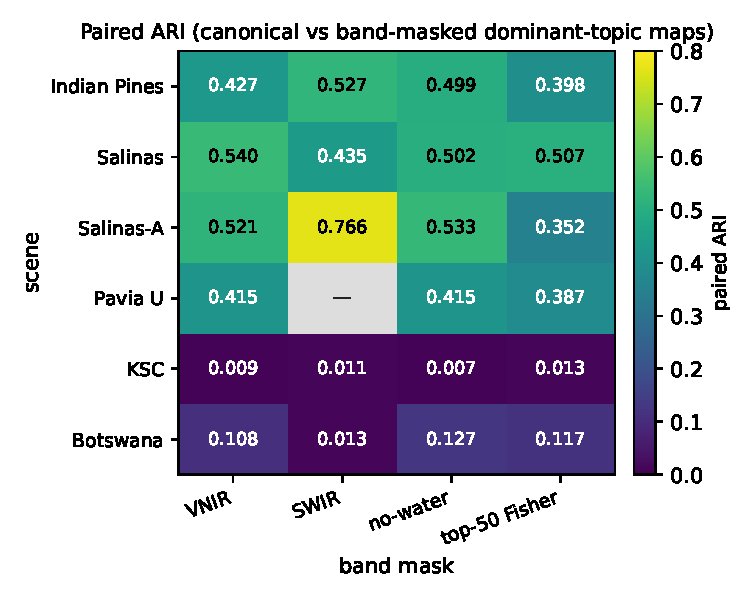
\includegraphics[width=\columnwidth]{paired-ari-heatmap.pdf}
\caption{F-5 paired ARI heatmap across (scene, mask) tuples. KSC
paired ARI sits at $0.007$--$0.013$ across all four masks
(band-fragile regime); Botswana shows a mixed pattern (SWIR $0.013$
band-fragile; VNIR $0.108$, no-water $0.127$, top-50 Fisher $0.117$
indicating partial structure under those masks); Salinas-A under
SWIR-only reaches $0.766$ (band-robust regime). The remaining tuples
fall in the partial-robustness range $0.35$--$0.54$. Pavia~U
$\times$ SWIR is auto-skipped (sensor is VNIR-only).}
\label{fig:paired-ari-heatmap}
\end{figure}

\begin{figure*}[t]
\centering
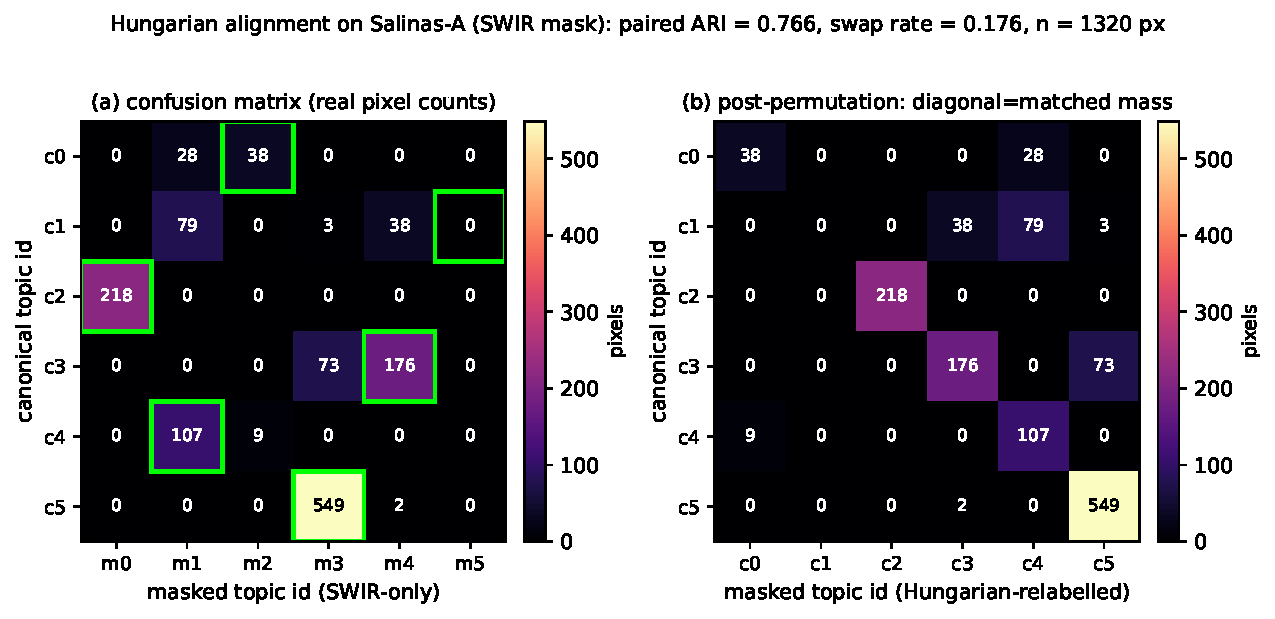
\includegraphics[width=0.8\textwidth]{hungarian-alignment-example.pdf}
\caption{F-8 Hungarian topic-id alignment on Salinas-A under SWIR-only
restriction. Lime rectangles mark the maximum-weight bipartite match
$\sigma^*$; the diagonal under permutation dominates, consistent with
the high paired ARI ($0.766$) and the low swap rate ($0.176$) on this
(scene, mask) tuple.}
\label{fig:hungarian-example}
\end{figure*}

Table~\ref{tab:b5-band-mask} and Fig.~\ref{fig:paired-ari-heatmap}
report the paired ARI across (scene,
mask) tuples on the six labelled scenes. The dominant observation is
the sharp split between \emph{band-fragile} and \emph{band-robust}
scenes. KSC paired ARI ranges from $0.007$ to $0.013$ across all four
masks: the masked LDA assigns pixels to topics with effectively
chance-level agreement with the canonical fit. Botswana sits in the
same regime only under SWIR ($0.013$); under VNIR ($0.108$), no-water
($0.127$) and top-50 Fisher ($0.117$) it reaches $0.11$--$0.13$, still
well below the labelled-scene average. The canonical-fit topic
identity on these scenes is \emph{not} recoverable from any
reasonable band subset. Salinas-A under SWIR-only restriction reaches
paired ARI $=0.766$: the masked fit recovers nearly the same
partition (Fig.~\ref{fig:hungarian-example}), indicating that the spectral signature carried by the
SWIR bands is sufficient to identify the canonical structure of this
scene.

\begin{table*}[t]
\caption{F-5 paired ARI per (scene, mask) tuple. Bold cells indicate
the band-mask that achieves the highest paired ARI per scene.
Pavia~U $\times$ SWIR is auto-skipped (sensor is VNIR-only).
Hungarian-aligned swap rates and per-topic alignments are in the
companion artefact \texttt{band\_masks/canonical\_comparison.json}.}
\label{tab:b5-band-mask}
\centering
\small
\begin{tabular}{lcccccccc}
\toprule
 & \multicolumn{4}{c}{Paired ARI} & \multicolumn{4}{c}{Bands kept of $B$} \\
\cmidrule(lr){2-5}\cmidrule(lr){6-9}
Scene & vnir & swir & no-water & top-50 & vnir & swir & no-water & top-50 \\
\midrule
Indian Pines     & 0.427 & \textbf{0.527} & 0.499 & 0.398 & 67/200 & 133/200 & 177/200 & 50/200 \\
Salinas          & \textbf{0.540} & 0.435 & 0.502 & 0.507 & 68/204 & 136/204 & 180/204 & 50/204 \\
Salinas-A        & 0.521 & \textbf{0.766} & 0.533 & 0.352 & 68/204 & 136/204 & 180/204 & 50/204 \\
Pavia University & \textbf{0.415} & --    & \textbf{0.415} & 0.387 & 103/103 & 0/103  & 103/103 & 50/103 \\
Kennedy Space C. & 0.009 & 0.011 & 0.007 & \textbf{0.013} & 59/176 & 117/176 & 155/176 & 50/176 \\
Botswana         & 0.108 & 0.013 & \textbf{0.127} & 0.117 & 49/145 & 97/145  & 127/145 & 50/145 \\
\bottomrule
\end{tabular}
\end{table*}

\subsection{F-6: cross-method clustering agreement}

Table~\ref{tab:b6-cross-method} reports the all-pairs ARI matrix on
Indian Pines. The dominant observation: the canonical topic-dominant
map has \emph{low} pairwise ARI against the spatial-segmentation
partitions (SLIC, Felzenszwalb, patches) but the label--topic ARI is
$0.203$, comparable to the SLIC-500-vs-label ARI $0.227$. The two
partitions are arriving at similar accuracy levels through different
inductive biases; the cross-method agreement matrix surfaces this in
a way that the per-method OA bar chart hides.

\begin{table*}[t]
\caption{F-6 cross-method ARI matrix on Indian Pines. Diagonal is
1.0 (omitted). Each entry is ARI(row, column). Label denotes the
ground-truth class map; topic-dominant denotes the canonical LDA
dominant-topic map. SLIC sizes correspond to target segment counts;
patches denote KMeans on flattened $7\times7$ or $15\times15$
spectral windows; pixel is the trivial identity partition.}
\label{tab:b6-cross-method}
\centering
\small
\begin{tabular}{lccccccc}
\toprule
                  & label & topic-dom. & felz. & SLIC-500 & SLIC-2000 & patch-15 & patch-7 \\
\midrule
label             & --    & 0.203      & 0.567 & 0.227    & 0.051     & 0.281    & 0.117 \\
topic-dominant    & 0.203 & --         & 0.120 & 0.039    & 0.010     & 0.047    & 0.021 \\
felzenszwalb      & 0.567 & 0.120      & --    & 0.306    & 0.076     & 0.372    & 0.170 \\
SLIC-500          & 0.227 & 0.039      & 0.306 & --       & 0.239     & 0.359    & 0.374 \\
SLIC-2000         & 0.051 & 0.010      & 0.076 & 0.239    & --        & 0.150    & 0.316 \\
patch-15          & 0.281 & 0.047      & 0.372 & 0.359    & 0.150     & --       & 0.292 \\
patch-7           & 0.117 & 0.021      & 0.170 & 0.374    & 0.316     & 0.292    & -- \\
\bottomrule
\end{tabular}
\end{table*}

\subsection{F-7 + F-8: topic--label coupling and per-topic identity}

We use the per-topic KL divergence
$\mathrm{KL}\!\big(P(L \mid t) \,\|\, P(L)\big)$ between the empirical
distribution of ground-truth labels conditioned on topic $t$ and the
marginal label distribution as a per-topic concentration measure;
the within-scene mean and max over the canonical-fit topics
are reported in Table~\ref{tab:b7-coupling}, computed from the
\texttt{kl\_to\_label\_prior\_per\_topic} field of
\texttt{topic\_to\_data/<scene>.json}.

\begin{table}[t]
\caption{F-7 topic--label coupling: per-topic
$\mathrm{KL}(P(L\mid t) \,\|\, P(L))$ mean and max on the
\emph{canonical fit} of each labelled scene (i.e.\ the no-mask
LDA fit). Higher values denote more sharply label-aligned topics.}
\label{tab:b7-coupling}
\centering
\small
\begin{tabular}{lcc}
\toprule
Scene & KL mean (nats) & KL max (nats) \\
\midrule
Indian Pines     & 1.35 & 2.51 \\
Salinas          & 1.73 & 2.77 \\
Salinas-A        & 1.29 & 1.79 \\
Pavia University & 0.81 & 1.17 \\
Kennedy Space C. & 0.95 & 2.50 \\
Botswana         & 1.73 & 3.37 \\
\bottomrule
\end{tabular}
\end{table}

\subsection{Combining F-5 and F-1: band-fragile or label-recoverable?}

A scene's appearance in the band-fragile regime (paired ARI
$\approx 0$) does not, by itself, imply low classifier accuracy on
that scene. Botswana paired ARI is $\approx 0.01$ on SWIR but the
mask-vs-label ARI on the same fit is $0.098$ (within range of
labelled-scene comparable values). The two metrics are measuring
different things: paired ARI(canonical, masked) asks whether the
canonical topic identities survive a band restriction, while
ARI(masked, label) asks whether the masked fit still discriminates
the classes. A band-fragile scene with a non-zero mask-vs-label ARI
is one on which the topic basis is being \emph{re-derived from
scratch} under each mask, with topic identity unstable but topic
discriminability preserved.

\subsection{Synthesis: per-scene model card}

Table~\ref{tab:summary} consolidates the per-scene values across
axes F-1, F-2, F-3, F-5, F-7 for the labelled scenes. We argue that this
synthesis, not the single OA number, is the appropriate unit of
reporting for a topic model on HSI.

\begin{table*}[t]
\caption{Per-scene model card synthesising the framework's main
axes. F-1 column: macro-F1 of \texttt{topic\_routed\_soft} (the
canonical topic-based classifier), mean of the five folds.
F-2: $c_v$ coherence of the canonical fit. F-3: single-seed
head-to-head KMeans-vs-label ARI of LDA. F-5: max paired ARI across the four masks (the
``best-case band-robustness''). F-7: per-topic
$\mathrm{KL}(P(L\mid t) \,\|\, P(L))$ mean over canonical-fit topics.}
\label{tab:summary}
\centering
\small
\begin{tabular}{lccccc}
\toprule
Scene & F-1 (macro-F1) & F-2 ($c_v$) & F-3 (ARI, 1 seed) & F-5 (max paired) & F-7 (KL nats) \\
\midrule
Indian Pines     & 0.839 & 0.450 & 0.287    & 0.527 & 1.35 \\
Salinas          & 0.954 & --    & --       & 0.540 & 1.73 \\
Salinas-A        & 0.996 & --    & --       & \textbf{0.766} & 1.29 \\
Pavia University & 0.819 & --    & --       & 0.415 & 0.81 \\
Kennedy Space C. & 0.921 & --    & --       & 0.013 & 0.95 \\
Botswana         & 0.962 & --    & --       & 0.127 & 1.73 \\
\bottomrule
\end{tabular}
\end{table*}

The F-1 column spans 0.819 (Pavia University) to 0.996 (Salinas-A),
and it does not track band robustness: the two band-fragile scenes,
Kennedy Space Center and Botswana (F-5 of 0.013 and 0.127), have the
fourth- and second-highest F-1.

% ---------------------------------------------------------------------
\section{Discussion}
\label{sec:discuss}
% ---------------------------------------------------------------------

\subsection{Why the band-mask diagnostic separates scenes}

The split between \emph{band-fragile} (KSC, Botswana) and
\emph{band-robust} (Salinas-A) scenes is, on its face, surprising:
KSC and Botswana have rich spectral signatures, broad spatial
coverage, and a comparable per-class sample budget to Salinas-A. Two
mechanisms are consistent with the diagnostic.

\emph{Mechanism (i): canonical topics exploit band-level redundancy.}
The canonical fit may be using fine-grained spectral co-variation
patterns that are present in the full-band representation and disappear
when half the bands are dropped. Under this mechanism the canonical
basis is not \emph{wrong}, but it is \emph{not transportable} across
spectral windows. Any claim of the form ``topic $k$ corresponds to a
specific land-cover signature'' presupposes a fixed reference frame
in which $\phi_k$ is defined; the diagnostic shows that on KSC and
Botswana this reference frame is band-window-conditional.

\emph{Mechanism (ii): the canonical topics are weakly identified.}
KSC has 13 classes and, at the canonical 220 samples per class,
$D = 2686$ documents; Botswana has 14 classes and $D = 2775$. The latent topic basis
$\phi$ has $K \times B \approx 12 \times 176$ free parameters on KSC.
With $D = 2686$ and a per-document token budget bounded by 13
quantisation levels times $B$ bands, the data-to-parameter ratio is
unfavourable; the posterior over $\phi$ has substantial mass over
many high-likelihood configurations, and a band restriction selects a
different posterior mode of the same family.

The diagnostic does not distinguish (i) from (ii); both are valid
warnings to a downstream consumer of the topic basis. The framework's
contribution is to make the warning legible.

\subsection{What the topic proportions lose}

A logistic regression on the topic proportions trails the raw-spectrum
baseline on both benchmark families: by 0.325 macro-F1 on the labelled
scenes (every one of the 30 scene--fold cells) and by 0.268 on the
HIDSAG targets (18 of 19). The deficit is therefore not specific to
mineralogical data. A $\theta$ of at most twelve proportions summarises
a spectrum of $B$ bands, and the narrow, locally discriminative
absorption features that separate classes (mineral classes on HIDSAG)
plausibly do not survive that compression; the raw multinomial
logistic keeps them. On the labelled
scenes the topic-routed classifiers, which use $\theta$ only to route
the raw spectrum to per-topic experts, match the baseline (a
difference of $+0.005$ for soft gating and $-0.001$ for hard gating).
The implication is that the topic representation is an interpretable
routing and summary layer rather than a replacement for the spectrum
as classifier input. Whether routing closes the gap on HIDSAG as it
does on the labelled scenes was not tested and is a direct follow-up.

\subsection{LDA versus ProdLDA versus ETM}

The ARI-vs-$c_v$ trade-off in Section~\ref{subsec:res-b3} bears on the
criterion on which ProdLDA was introduced as an improvement over LDA,
higher topic coherence on text corpora~\cite{srivastava2017autoencoding},
a claim made for its product-of-experts decoder. On Indian Pines the
amortised mixture-decoder model labelled ProdLDA here also has the
highest coherence (ProdLDA $c_v = 0.630$ vs LDA $c_v = 0.450$ vs ETM
$c_v = 0.357$), but the cluster-ARI ordering inverts (LDA $0.287$ vs
ETM $0.257$ vs ProdLDA $0.165$). The coherence-vs-clustering
disagreement is, on HSI, large enough to flip the practitioner-level
recommendation: a practitioner who picks ProdLDA because its
coherence is highest will obtain a topic basis that clusters worst
against ground truth. We therefore recommend, for HSI specifically,
reporting both metrics side-by-side rather than choosing one as
representative.

\subsection{Limitations}

The framework has three operative limitations. \emph{First}, the
canonical fit uses a single $K$ per scene, chosen by the formula
$K = \max(4, \min(12, n_{\text{classes}}))$. A more sensitive analysis
would sweep $K$ and report per-axis behaviour against $K$; we report
the $K$-sweep on F-4 but other axes are computed at the canonical $K$.
\emph{Second}, the tokenisation $Q+1 = 13$ levels is uniform across
scenes, not adapted to per-scene spectral dynamic range. \emph{Third},
F-12 matches topics to library categories by cosine similarity alone:
a high cosine indicates spectral plausibility, not a mineralogical
identification, and the paper does not compare against published
accuracies, whose train/test splits would not match the splits used
here.

% ---------------------------------------------------------------------
\section{Reproducibility artefacts}
\label{sec:repro}
% ---------------------------------------------------------------------

The full reproducibility package consists of:

{\raggedright
\begin{itemize}
\item \textbf{Builder source.} Forty-plus deterministic Python
builders under \path{data-pipeline/builders/}, each accepting a
fixed seed and writing a deterministic JSON or NPZ artefact under
\path{data/derived/}. Each builder records its
\path{builder_version} and \path{generated_at} ISO timestamp in
the artefact metadata.
\item \textbf{Derived artefacts.} 3895 JSON and binary files,
449~MB total, including: per-scene canonical fits
(\path{theta_grid.bin}, \path{dominant_topic_map.bin}), the
band-mask canonical comparison
(\path{band_masks/canonical_comparison.json}, the source of all
F-5 numbers above), the cross-method agreement matrices
(\path{cross_method_agreement/}), the seed-stability sweeps
(\path{neural_topic_seed_stability/}), the hierarchical Bayesian
posteriors
(\path{method_statistics_labelled/cross_classification_bayesian.json}
and \path{method_statistics_hidsag/cross_classification_bayesian.json}),
and the HIDSAG cross-preprocessing stability sweeps.
\item \textbf{Web application.} A FastAPI backend serving the
artefacts over 59 REST endpoints, plus a React+Vite frontend at
\url{https://lda-hsi.fasl-work.com} that consumes them as interactive
visualisations.
\item \textbf{Endpoint test harness.} A test script covering 109
endpoints that verifies endpoint health, response schemas, and the
content of the single-page-application shell at each deployment.
\item \textbf{Companion paper.} The F-5 band-mask diagnostic is reported
in detail in~\cite{santibanezleal2026bandmask}.
\end{itemize}
\par}

All code is MIT-licensed at
\url{https://github.com/fsantibanezleal/CAOS_LDA_HSI}.

% ---------------------------------------------------------------------
\section{Conclusion}
\label{sec:conclude}
% ---------------------------------------------------------------------

The accuracy-only view of topic models on hyperspectral imagery
hides the questions an interpretability-motivated practitioner most
needs answered: is the topic basis reproducible across seeds,
robust to spectral-window choice, calibrated against label entropy,
actually outperforming linear baselines, and consistent across
preprocessing recipes? We propose a twelve-axis evaluation framework
that returns one operational metric per axis and stores each metric as
a deterministic JSON artefact. Applied to six labelled HSI benchmarks
and five HIDSAG mineralogical subsets, the framework surfaces three
findings the accuracy-only view does not: the topic-routed soft
classifier matches the raw-spectrum logistic baseline on the labelled
scenes (0.915 against 0.910 macro-F1); the
band-mask diagnostic separates scenes whose canonical topics are
band-robust (Salinas-A SWIR paired ARI $0.766$) from scenes whose
topics are band-fragile (KSC under every mask and Botswana under SWIR,
paired ARI $\approx 0.01$);
and a classifier on the topic proportions alone trails the raw-spectrum
baseline on both the labelled scenes (by 0.325 macro-F1) and the HIDSAG
targets (by 0.268). The full 3895-artefact
reproducibility package is released under MIT licence.

Future work includes (i) a per-axis $K$-sweep extending the
single-$K$ canonical fit, (ii) per-scene tokenisation budgets adapted
to spectral dynamic range, (iii) extending the framework to neural
unmixing variants (autoencoder unmixing, transformer-based topic
models), and (iv) developing an information-theoretic
within-mask Fisher complement to F-5 that does not depend on the
unmasked-spectrum ranking.

% ---------------------------------------------------------------------
\section*{Acknowledgements}
% ---------------------------------------------------------------------

This work has been partially funded by The Advanced Mining Technology
Center (AMTC) Basal project (ANID/PIA Project AFB220002) and ANID
FONDECYT Postdoctorado 3220094.

The Hyperspectral Remote Sensing Scenes collection is maintained by
the Computational Intelligence Group at UPV/EHU. The HIDSAG
mineralogical database was the result of a collaboration on
hyperspectral mineralogy with industrial partners in Chilean mining
geosciences. The author thanks the open-source maintainers of
scikit-learn \cite{pedregosa2011scikit}, NumPy \cite{harris2020numpy},
SciPy \cite{virtanen2020scipy}, and Gensim \cite{rehurek2010gensim},
whose work this study rests on.

% ---------------------------------------------------------------------
\section*{Conflict of Interest}
% ---------------------------------------------------------------------

The author is a co-author of the HIDSAG dataset descriptor
publication~\cite{hidsag2023} and the accompanying data
release~\cite{hidsag2023figshare}, and first author of the
earlier conference paper introducing the LDA-V1/V2/V3 corpus
recipes and topic-routed regressor on private geometallurgical
data~\cite{santibanezleal2022procemin}. The present paper
is methodologically distinct: it proposes a twelve-axis evaluation
framework for topic models on hyperspectral imagery and applies
the framework, among other benchmarks, to the HIDSAG mineralogical
subsets. HIDSAG is cited as a data source, not as a methodological
contribution of this work. The author declares no other conflict
of interest.

% ---------------------------------------------------------------------
\section*{Data Availability Statement}
% ---------------------------------------------------------------------

All numerical results in this paper derive from deterministic
artefacts under \texttt{data/derived/} in the companion code
repository at \url{https://github.com/fsantibanezleal/CAOS_LDA_HSI}.
The paired F-1 comparisons of Tables~\ref{tab:b1-labelled}
and~\ref{tab:b1-hidsag} are computed from
\path{topic_routed_classifier/} and \path{core/local_core_benchmarks.json}
by \path{figures/source/build_bayesian_method_comparison.py} of the
manuscript repository
\url{https://github.com/fsantibanezleal/CAOS_LDA_HSI_Paper}.
The HIDSAG database is available from
\cite{hidsag2023figshare}; the labelled hyperspectral benchmark
scenes (Indian Pines, Salinas, Salinas-A, Pavia U, KSC, Botswana)
are available from the UPV/EHU Hyperspectral Remote Sensing Scenes
collection \cite{baumgardner1992indianpines,aviris_salinas,rosis_pavia,aviris_ksc,eo1_botswana}.
The 3895-artefact derived bundle, the
\texttt{build\_*.py} pipeline source, the FastAPI backend, and the
React frontend are released under the MIT licence. The interactive
demonstration is hosted at
\url{https://lda-hsi.fasl-work.com}.

% ---------------------------------------------------------------------
\bibliographystyle{IEEEtran}
\bibliography{../../bibliography/refs,companion}
% ---------------------------------------------------------------------

\end{document}
